
%(BEGIN_QUESTION)
% Copyright 2012, Tony R. Kuphaldt, released under the Creative Commons Attribution License (v 1.0)
% This means you may do almost anything with this work of mine, so long as you give me proper credit

A water-cooled generator at a power plant has two sources of cooling water flow, each source equipped with a flow switch that returns to its normal status (open) if the water flow through the pipe drops to too low of a rate:

$$\includegraphics[width=15.5cm]{i03198x01.eps}$$

\vskip 10pt

Classify the alarm and the shutdown functions, each using {\it MooN} notation.

\vskip 10pt

Given the following component dependabilities (and neglecting all other dependabilities in the system such as the power source), calculate the dependability of the alarm function and also the dependability of the shutdown function:

\begin{itemize}
\item{} Dependability of each flow switch = 0.993
\item{} Dependability of each control relay = 0.9991
\item{} Dependability of lamp = 0.998
\item{} Dependability of shutdown solenoid = 0.965
\end{itemize}

\vskip 10pt

Supposing you were assigned the task of testing this alarm/shutdown system as thoroughly as possible without actually interrupting water flow through either of the cooling water pipes, or actually shutting the generator down, design a testing procedure to determine as much as possible the readiness of this alarm/shutdown system.  Points to identify in your procedure:

\begin{itemize}
\item{} Any electrical connections you would need to temporarily break
\item{} Any temporary ``jumper'' connections you would need to make
\item{} What you would detect or measure as confirmation that the system works as designed
\item{} The order in which all steps would need to be done
\end{itemize}

\filbreak

\vskip 20pt \vbox{\hrule \hbox{\strut \vrule{} {\bf Suggestions for Socratic discussion} \vrule} \hrule}

\begin{itemize}
\item{} Identify any safety precautions to follow when working on a ``live'' 120 VAC circuit (e.g. the {\it one-hand} rule).
\item{} Are the flow switches' {\it normal} state the same as their {\it typical} state when the system is running as it should?  Explain the distinction between ``normal'' and ``typical'' in this context.
\end{itemize}

\underbar{file i03198}
%(END_QUESTION)





%(BEGIN_ANSWER)

This system provides 1oo2 alarm and 2oo2 shutdown functions.

\vskip 10pt

Probability calculations using logic symbols:

$$\includegraphics[width=15.5cm]{i03198x02.eps}$$

%(END_ANSWER)





%(BEGIN_NOTES)

\noindent
{\bf Trip test procedure (in order):}

\begin{itemize}
\item{} Disconnect wire at TP9 or TP10 (disables shutdown solenoid)
\item{} Connect voltmeter between TP9 and TP10 
\item{} Disconnect wire at either TP1 or TP2 -- alarm light should come on
\item{} Reconnect wire (TP1 or TP2) -- alarm light should turn off
\item{} Disconnect wire at either TP3 or TP4 -- alarm light should come on
\item{} Disconnect wire at either TP1 or TP2 -- voltmeter should register supply voltage
\item{} Reconnect wires (TP1 or TP2; TP3 or TP4)
\item{} Remove voltmeter from circuit
\item{} Reconnect wire at TP9 or TP10 (enables shutdown solenoid)
\end{itemize}


\vskip 20pt \vbox{\hrule \hbox{\strut \vrule{} {\bf Virtual Trip-testing} \vrule} \hrule}

This question is a good candidate for a ``Virtual Trip-testing'' exercise.  Presenting the diagram to students, you pose an assignment whereby students must figure out how to test some component of this system to check that it will operate as intended to shut down the system in an abnormal (trip) condition, with some realistic limitation (e.g. power cannot be shut off to the load).  Students then propose various methods for executing the test.  Your job is to determine whether or not their proposed tests will achieve the desired result(s).

During and after the exercise, it is good to ask students follow-up questions such as:

\begin{itemize}
\item{} Where might our planned test strategy go wrong?  In other words, what thing(s) might happen to foil our test, either to invalidate the results or to not honor the stated limitation(s)?
\item{} Suppose the limitation were different.  How would this affect our ability to carry out the test?
\item{} Is the last test strategy best one we could execute?
\end{itemize}


%INDEX% Safety, shutdown system: trip testing
%INDEX% Switch, flow
%INDEX% Troubleshooting review: electric circuits

%(END_NOTES)


